\documentclass[sigconf]{acmart}

\usepackage{booktabs} % For formal tables


% Copyright
%\setcopyright{none}
%\setcopyright{acmcopyright}
%\setcopyright{acmlicensed}
\setcopyright{rightsretained}
%\setcopyright{usgov}
%\setcopyright{usgovmixed}
%\setcopyright{cagov}
%\setcopyright{cagovmixed}


% DOI
\acmDOI{10.475/123_4}

% ISBN
\acmISBN{123-4567-24-567/08/06}

%Conference
\acmConference[SC17]{SuperComputing}{November 2017}{Denver, Colorado, USA} 
\acmYear{1997}
\copyrightyear{2017}

\acmPrice{15.00}


\begin{document}
\title{High-level python abstractions for optimal checkpointing in inversion problems}
%\titlenote{Produces the permission block, and
%  copyright information}
%\subtitle{Checkpointing, done beautifully.}
%\subtitlenote{The full version of the author's guide is available as
%  \texttt{acmart.pdf} document}


\author{Navjot Kukreja}
\authornote{Note: Author list is not finalized yet. Subject to change}
\affiliation{%
  \institution{Imperial College London}
  \city{London}
  \country{UK}}
\author{Jan H\"uckelheim}
\affiliation{%
  \institution{Imperial College London}
  \city{London}
  \country{UK}}
\author{Michael Lange}
\affiliation{%
  \institution{Imperial College London}
  \city{London}
  \country{UK}}
\author{Andrea Walther}
\affiliation{%
  \institution{Universit\"at Paderborn}
  \city{Paderborn}
  \country{Germany}}

\renewcommand\shortauthors{Kukreja, N. et al}

\begin{abstract} TODO
The computation of adjoints in optimisation and inverse design problems requires storing
intermediate data. The available memory size sets a limit to this, and necessitates recomputation in
some instances. Revolve checkpointing offers an optimal schedule that trades computational cost for
smaller memory footprints. Integrating Revolve into a modern python HPC code and combining it with
code generation is not straightforward. We present an API that makes checkpointing accessible from a
DSL-based code generation environment and present a benchmark study. TODO.
\end{abstract}

%
% The code below should be generated by the tool at
% http://dl.acm.org/ccs.cfm
% Please copy and paste the code instead of the example below. 
%
\begin{CCSXML}
<ccs2012>
<concept>
<concept_id>10011007.10011074.10011075.10011077</concept_id>
<concept_desc>Software and its engineering~Software design engineering</concept_desc>
<concept_significance>500</concept_significance>
</concept>
</ccs2012>
\end{CCSXML}

\ccsdesc[500]{Software and its engineering~Software design engineering}
%
% End generated code
%


\keywords{HPC, Code generation, API, Checkpointing, Adjoint, Inverse Problems}


\maketitle

\section{Introduction}
(1 page)
Seismic inversion, and more specifically Full Waveform Inversion (FWI)
is a computationally heavy technique that uses data from seismic wave
propagation experiments to calculate physical parameters of the
earth's subsurface. In case of FWI, this additional information on the
physical parameters drives the generation of better subsurface
images (CITE). An FWI problem is setup as an optimization problem using
a gradient-based optimization algorithm with the objective function
being minimised is the misfit between the simulated data and the
observed data received at the receivers. A finite-difference
discretization of one of the forms of the wave equation acts as the
constraint for the optimization. Since the gradient is calculated using the
adjoint-state method, by the correlation between the fields in forward
and adjoint (reverse) mode (CITE), the method requires that the forward and
adjoint field be known for each time step in the
simulation. Considering that the typical domain for such a setup is 3
dimensional with 1000 points in each dimension, the field requires
$1000 \times 1000 \times 1000 \times 4 = 4 \times 10^{9} $ bytes ( 4
GB) of memory for a single timestep. Since the simulation is run for a
typical $3000$ time-steps, storing the entire forward field in memory
would require $12 TB$ of memory which is prohibitively high. We
discuss this in section \ref{sec:inversion_devito}. 

Previous work on similar inverse problems led to the \emph{Revolve}
algorithm \cite{griewank2000} and the associated C++ tool which
provides an optimal schedule at which to store checkpoints,
i.e. states from which the forward simulation can be restored. This
algorithm is further discussed in section \ref{sec:revolve}.

The tool and the algorithm, however, only provide the schedule to be
used for checkpointing. Although this eases some of the complexity of
the application code using the algorithm, the glue code required to
manage the forward and adjoint runs is still quite complex. This acts
as a deterrent to more widespread use of the algorithm in the
community. 

In this paper we describe how the algorithm can be combined with code
generation to make checkpointing much more accessible. The software that
can enable this is described in section \ref{sec:api}. 

The performance impact of using the checkpointing scheme, as well as
the effect of the size of memory available is studied in section
\ref{sec:experiment}. 

Motivation: Why do we need to connect revolve and a python seismic inversion code? What is there to
learn for others? How does our work help readers and the world?

\section{Seismic inversion and Devito}
(1 page)
\label{sec:inversion_devito}
Some context on seismic imaging, the PDEs, the method. Why use
adjoints. Why is this problem time-dependent. Why do we need a lot of
data.
Code generation, references to previous papers about Devito. Why not
be brave and write this in Fortran.

\section{Revolve}
(2 pages)
\label{sec:revolve}
How does revolve work and save memory, how is it implemented in C++. What other variants (online,
multi-stage) are in the implementation.

\section{API: Connecting Revolve with Devito}
(3 pages)
\label{sec:api}
This is the core of the paper.

What distinguishes us from previous work? What are our aims?
\begin{itemize}
\item The user (domain-specialist) can write high-level python code that gets translated into low
level code. The high-level code defines the PDE, but typically has nothing like loops etc.
\item Users define PDEs for primal and adjoint, both get compiled into efficient code.
\item How to make checkpointing available without forcing user to interfere with loops, callbacks,
data storage mechanisms? Basically, the user should choose whether to use checkpointing in one
place, but not be forced to to anything beyond this.
\item How to design an interface so that all knowledge of checkpointing, different strategies
(online/offline checkpointing, multistage) are contained within one module of the python framework,
and still benefits all operations in the code?
\item How to integrate checkpointing into the simulation (a mix of generated, highly efficient C
code and Python) without polluting all code?
\end{itemize}

This work showcases pyrevolve, a new python library developed by us, that provides a python
interface to Revolve. This library was integrated into the Devito code generation framework.

The pyrevolve library contains two parts: crevolve, which is a thin Python wrapper around a
previously published C++
implementation\footnote{http://www2.math.uni-paderborn.de/index.php?id=12067\&L=1}, and pyrevolve
itself, which sits on top of crevolve and manages data and computation management for the user.

The C++ files in this package are slightly modified to play more nicely with Python, but the
original is available from the link below. In addition, there is a C wrapper around the C++ library,
to simplify the interface with Python. This C wrapper is taken from
libadjoint\footnote{https://bitbucket.org/dolfin-adjoint/libadjoint}.

The major change is that pyrevolve is no longer responsible for performing the data copies, and
therefore no longer needs to know about the properties of Devito symbols, or which of those need to
be stored. The user must give to pyrevolve an object that knows about the size of a single
checkpoint, and has a routine to deep-copy all required live-data into a given memory location, or
to load data from such a memory location into the live symbols so that the operators can resume the
computation.

\subsection{API, Devito side}

To introduce checkpointing, Devito requires some additional features.

Following from the last discussion, this is to document the changes that will be made in Devito to
enable the use of checkpointing:

Start and stop Operators at a given time-step: Add optional parameters to Operator.apply() called
tstart and tend to (re)start the Operator from a given time-step and run for a given number of time
steps.

Store last accessed time step in data objects: This is largely related to issue \#69 where, when a
TimeData object has a buffered time dimension, it is not clear which buffer holds the field computed
at the last time-step. Currently we are working around this by externally tracking the number of
time-steps that were run on the object. This should be internalised so that external code can
reliably know how to access the last computed field. There was a proposal to do the same for
PointData objects as well but I don't remember the argument for that - could potentially be
discussed (again).

Deep copy routines inside symbolic data objects: All symbolic data objects to have a save routine to
save their state (data as well as the internal time counter added by the above, to start with) in a
memory location provided by the caller. There would also be an accompanying restore method to
restore state from a provided memory location. A corollary to this would be that a symbol should be
aware of and be capable of reporting the amount of memory required to save its state. This knowledge
would eventually find its way into the checkpointer which would be responsible for allocating memory
to store the checkpoints.

\subsection{API, Pyrevolve side}

pyrevolve will provide an abstract base class "Checkpoint" that must be extended by a user of
pyrevolve, and must provide

\begin{itemize}
\item a `size` property, containing the size of a checkpoint in Bytes,
\item a `save(ptr)` method that deep-copies all live data that needs to be checkpointed into the
provided location inside the Checkpoint storage, and
\item a `load(ptr)`method that deep-copies all data from the given location back into the live data.
\end{itemize}

To implement this Checkpoint class, a user will require the symbol deep\_copy routine. In addition,
pyrevolve requires that the operators accept `t\_start` and `t\_end` parameters, and can resume
their operation on the live data without confusing the state of the buffer. This is described in the
related issue https://github.com/opesci/devito/issues/247.

The actual computation will operate like this:

\begin{enumerate}
\item The user initialises the operators with whatever symbols are required, and implements a
concrete
implementation of the Checkpoint object with the above properties.
\item The user calls pyrevolve, with the arguments: `fwd\_operator`, `rev\_operator`, `checkpoint`,
`n\_time\_steps`, `n\_checkpoints`. (Other options will follow in the future and require a more
flexible interface, e.g. online checkpointing will no longer require `n\_time\_steps` upfront,
multistage checkpointing will require a list of `n\_checkpoints` along with relative speeds, etc.).
\item On initialisation, pyrevolve will query `checkpoint.size` for the size of one checkpoint, and
allocate `n\_checkpoints*checkpoint.size` bytes of memory for checkpoint storage.
\item Repeatedly, pyrevolve will call either of the following actions in the user-defined Checkpoint
and operators: `fwd\_operator.apply(tstart, tend)`, `rev\_operator.apply(tstart, tend)`,
`checkpoint.save(ptr)`, `checkpoint.load(ptr)`, where `ptr` will point to the start of the
appropriate checkpoint in the storage.
\item pyrevolve may in the future use multi-stage checkpointing to swap checkpoints to disk
(asynchronously?), but `ptr` as passed to `checkpoint.save` or `checkpoint.load` is guaranteed to
point to a checkpoint that is available in memory.
\end{enumerate}


\section{Test case, Results}
(2 pages)
\label{sec:experiment}
A nice test case that can be scaled up in size easily. Timings for different mesh sizes, with
different amounts of memory set as the upper limit.

We will use Marmousi 2D data, resampling it for different grid
resolutions. 

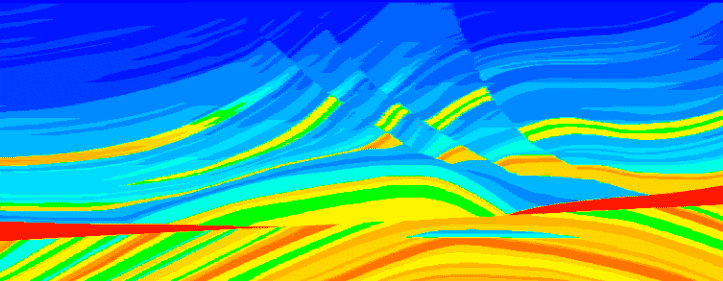
\includegraphics[width=0.8\linewidth]{images/marmousi_velocity.png} 

\section{Conclusions}
(1 page)
This work was highly successful, but more work could be done.

\begin{acks}
  The authors are very grateful to Mathias Louboutin (?), Simon Funke
  (?). 
\end{acks}


\bibliographystyle{ACM-Reference-Format}
\bibliography{bib_checkpointing} 

\end{document}
